\chapter{Conceptos de autonomía}
\label{cap:conceptos-autonomia}

\begin{enpocas}
Qué significa que un dron sea autónomo, el ciclo percibir--decidir--actuar, las máquinas de estados,
cómo se planea recorrer toda una zona, cómo se ubica algo que se ve, qué es el GPS y cómo se pasa de
metros a latitud y longitud, qué es un LiDAR y cómo se esquivan obstáculos.
\end{enpocas}

\section{Percibir, decidir, actuar}

Un dron autónomo repite sin parar tres pasos:
\begin{figure}[H]
\centering
\begin{tikzpicture}[blq/.style={draw,rounded corners,fill=#1,minimum width=3.2cm,minimum height=1.1cm,align=center},
  fl/.style={-{Stealth[length=2.5mm]},very thick}]
  \node[blq=blue!12] (p) at (0,0) {\textbf{Percibir}\\cámara, YOLO, LiDAR,\\odometría};
  \node[blq=green!12] (d) at (5,0) {\textbf{Decidir}\\máquina de estados,\\ruta, estimación};
  \node[blq=red!10] (a) at (2.5,-2.6) {\textbf{Actuar}\\consigna $\rightarrow$\\controlador $\rightarrow$ motores};
  \draw[fl] (p) -- (d); \draw[fl] (d) -- (a); \draw[fl] (a) -- (p);
\end{tikzpicture}
\caption{El ciclo de la autonomía. En nuestra simulación se repite 50 veces por segundo.}
\end{figure}
En nuestro caso: \emph{percibir} es mirar con la cámara y el LiDAR; \emph{decidir} es elegir a dónde
ir (seguir la ruta, acercarse al humo, rodear un árbol); \emph{actuar} es mandar la consigna al
controlador, que mueve los motores.

\section{Máquinas de estados}

Un comportamiento complejo se organiza en \textbf{estados}: en cada momento el dron está en uno
(``patrullando'', ``acercándose al foco''...), hace lo que ese estado indica y cambia a otro cuando se
cumple una condición (``vi humo en tres imágenes seguidas'').

\begin{ejemplo}
Un semáforo es una máquina de estados: verde $\rightarrow$ (pasan 30~s) $\rightarrow$ amarillo
$\rightarrow$ (pasan 3~s) $\rightarrow$ rojo $\rightarrow$ ... Una lavadora también: llenar, lavar,
enjuagar, centrifugar.
\end{ejemplo}

La búsqueda del incendio tiene siete estados (figura~\ref{fig:estados}): despegue, patrulla,
hacia\_humo, aproximación, verificación, descenso y órbita. Es fácil de entender, de probar y de
explicar, y cuando algo falla el registro dice en qué estado estaba.

\section{Planear la cobertura: recorrer todo el bosque}

Si no sabemos dónde está el incendio, hay que mirar todo. Eso es un problema de \textbf{planificación
de cobertura}: encontrar una ruta que haga pasar la ``huella'' de la cámara por toda la zona. La
solución clásica es ir y venir en franjas paralelas, como al podar un jardín (en inglés,
\emph{boustrophedon}: ``como gira el buey al arar''). Lo que importa es la \textbf{separación} entre
franjas: tan grande como se pueda (ruta más corta) pero sin dejar huecos sin ver.

\begin{figure}[H]
\centering
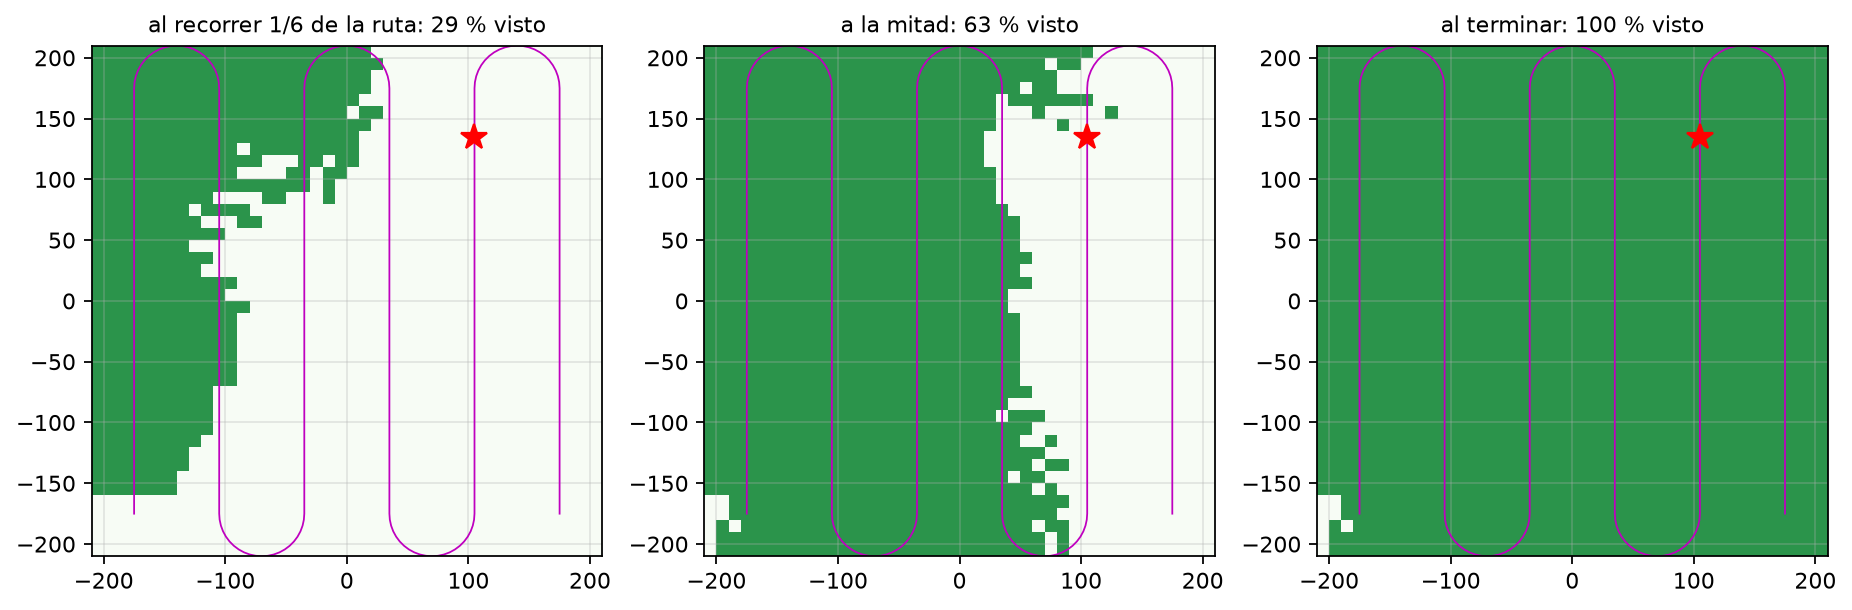
\includegraphics[width=\textwidth]{c_cobertura.png}
\caption{Simulación de qué tanto del bosque (celdas de 10~m) ha visto la cámara a lo largo de la
serpentina, a 30~m sobre el suelo y viendo hasta 150~m. La estrella roja es el incendio.}
\end{figure}

Durante el vuelo, el planificador lleva este mismo mapa (``cobertura'') y lo publica para verlo en
RViz.

\section{Ubicar lo que se ve}

Del capítulo~\ref{cap:imagen} sabemos que un píxel da una dirección. Para pasar a un punto del mapa hay dos caminos:

\textbf{Cortar el rayo con el terreno.} Si conocemos el relieve (un \textbf{modelo digital de
elevación}, DEM: una tabla con la altura del suelo cada 4~m), avanzamos por el rayo hasta que queda
por debajo del suelo. Así se estima la posición de las llamas.
\begin{figure}[H]
\centering
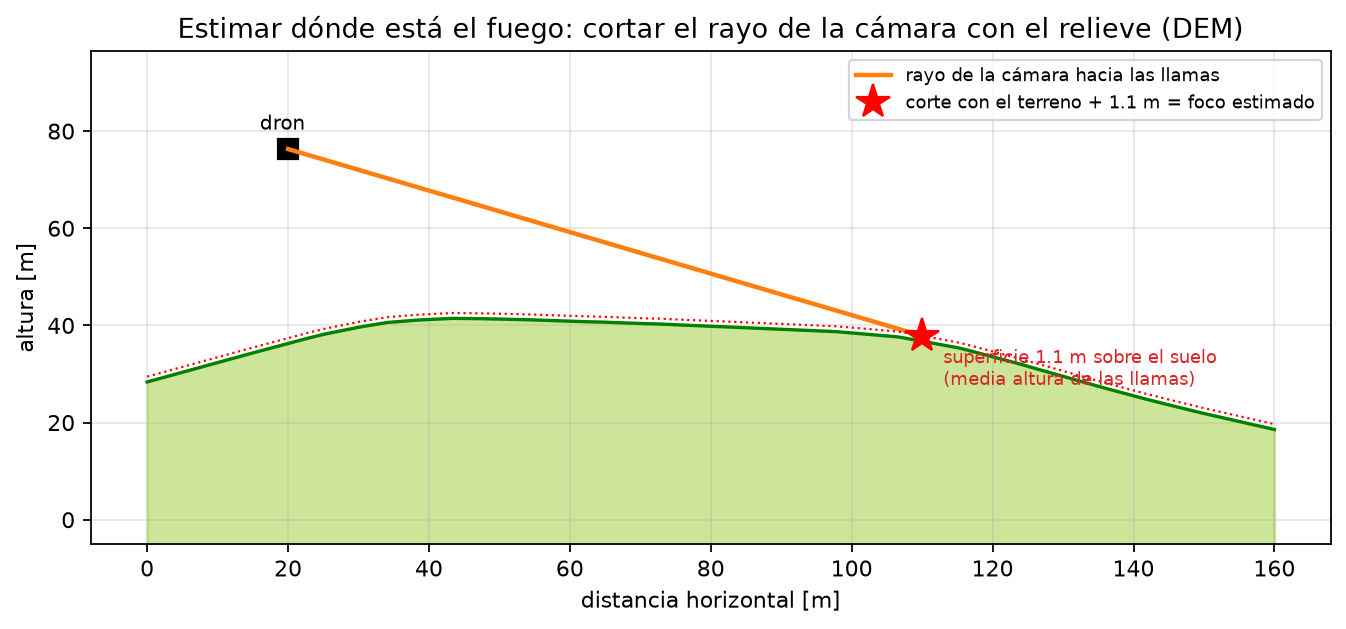
\includegraphics[width=0.9\textwidth]{c_rayo.png}
\caption{El rayo de la cámara hacia las llamas se corta con la superficie que está 1.1~m sobre el
relieve.}
\end{figure}

\textbf{Triangular.} El humo sube en columna vertical: verlo da la dirección hacia el foco pero no la
distancia. Con varias direcciones desde lugares distintos, el foco está donde se cruzan. Como las
mediciones tienen ruido, las rectas no se cruzan en un solo punto y se busca el más cercano a todas
(mínimos cuadrados).
\begin{figure}[H]
\centering
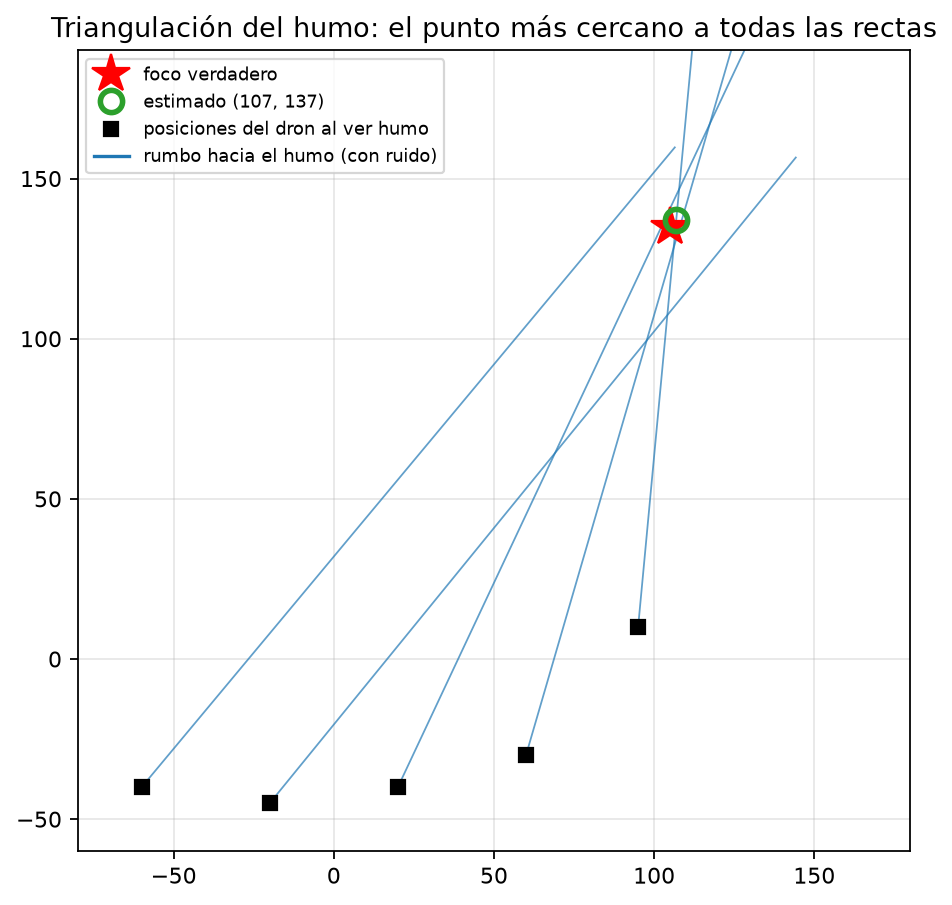
\includegraphics[width=0.7\textwidth]{c_triangulacion.png}
\caption{Triangulación del humo con cinco direcciones con ruido.}
\end{figure}

\begin{aviso}
La triangulación funciona mal si las direcciones son casi paralelas (todas vistas desde puntos
alineados en la misma dirección): un error pequeño en el ángulo mueve mucho el cruce. Por eso en la
simulación una estimación hecha solo con humo no basta para confirmar un incendio: el dron se acerca
hasta ver las llamas.
\end{aviso}

\section{GPS: de metros a latitud y longitud}

La simulación trabaja en metros sobre un plano (ENU), pero los bomberos necesitan
\textbf{coordenadas GPS}: latitud (cuánto al norte o sur del ecuador), longitud (cuánto al este u
oeste de Greenwich) y altitud. La Tierra no es una esfera sino un \textbf{elipsoide} un poco achatado;
el GPS usa el modelo \textbf{WGS84}.

\begin{figure}[H]
\centering
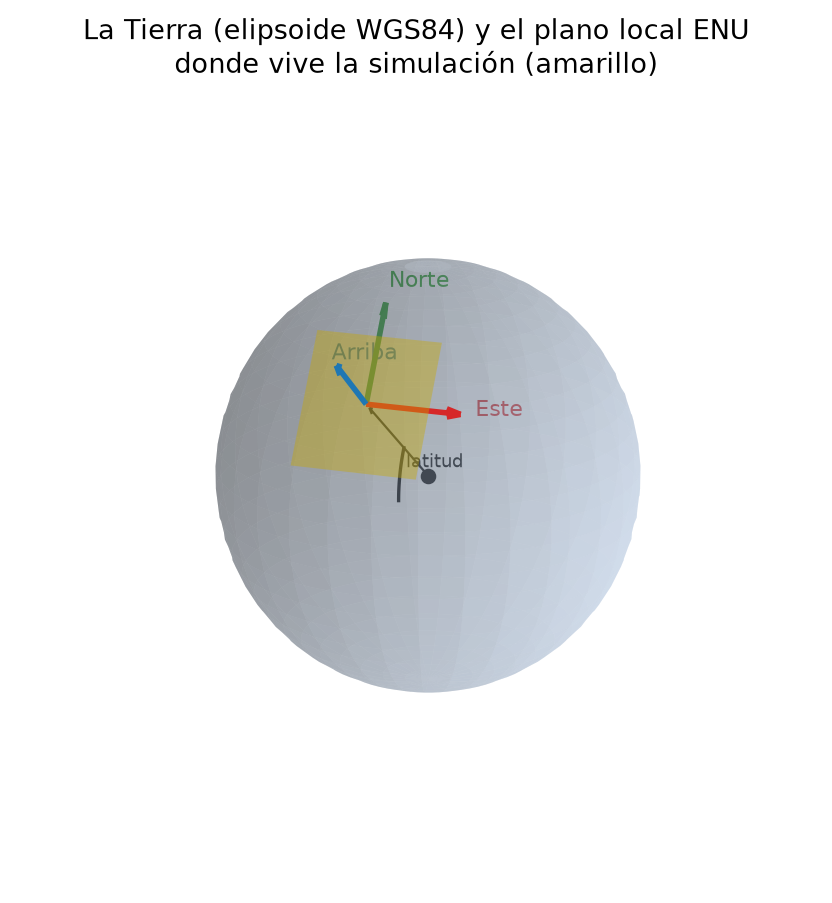
\includegraphics[width=0.6\textwidth]{c_tierra.png}
\caption{El plano local ENU de la simulación es tangente a la Tierra en el origen del mundo.}
\end{figure}

Para convertir se fija dónde está el origen del mundo (como supuesto, en el Parque Nacional Desierto
de los Leones, CDMX: 19.293° N, 99.311° O, 3000~m) y se hace la cuenta exacta: ENU $\rightarrow$
coordenadas cartesianas centradas en la Tierra (ECEF) $\rightarrow$ latitud, longitud y altitud
(sección~\ref{sec:gps}).

\begin{tecnico}
A esta latitud, un grado de latitud mide unos 110.8~km y uno de longitud unos 105.1~km. Por eso un
error de $10^{-6}$ grados en las coordenadas equivale a unos 10~cm: con seis decimales basta.
\end{tecnico}

\section{LiDAR: medir distancias con luz}

Un \textbf{LiDAR} lanza pulsos láser en muchas direcciones y mide cuánto tardan en regresar; con eso
calcula la distancia al primer obstáculo en cada dirección. El resultado es una \textbf{nube de
puntos}. El del dron simulado lanza 120 rayos alrededor por 16 alturas distintas, 10 veces por
segundo, hasta 30~m.

\begin{figure}[H]
\centering
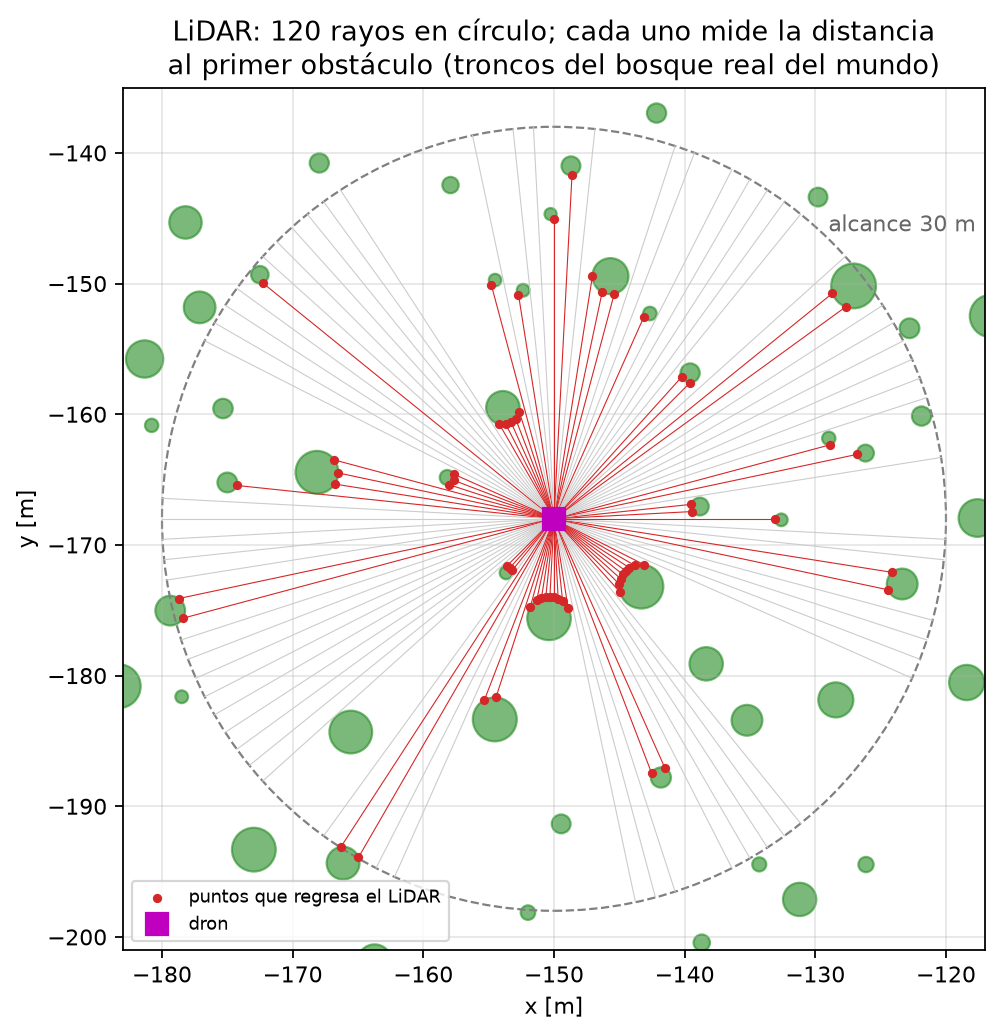
\includegraphics[width=0.6\textwidth]{c_lidar.png}
\caption{Una capa del LiDAR en el bosque del mundo grande: los rayos rojos tocan un tronco, los grises
no encuentran nada en 30~m.}
\end{figure}

A diferencia de la cámara, el LiDAR sí da distancias, pero no sabe ``qué'' es cada punto. Se
complementan: la cámara para reconocer el fuego, el LiDAR para no chocar.

\section{Evitar obstáculos}

Hay dos grandes familias de métodos:
\begin{description}
  \item[Planificación global:] con un mapa completo, se calcula de antemano una ruta sin choques
        (algoritmos como A* o RRT).
  \item[Evasión reactiva:] con lo que se ve en ese momento, se corrige el rumbo sobre la marcha.
        Es lo que hacemos: no tenemos un mapa de los árboles, solo lo que ve el LiDAR.
\end{description}
Nuestro método es del tipo \textbf{VFH} (\emph{vector field histogram}): se divide el círculo de
direcciones alrededor del dron en 72 sectores, se marcan los que están bloqueados por algún obstáculo
cercano y se elige el sector libre más parecido a la dirección a la que queremos ir.

\begin{figure}[H]
\centering
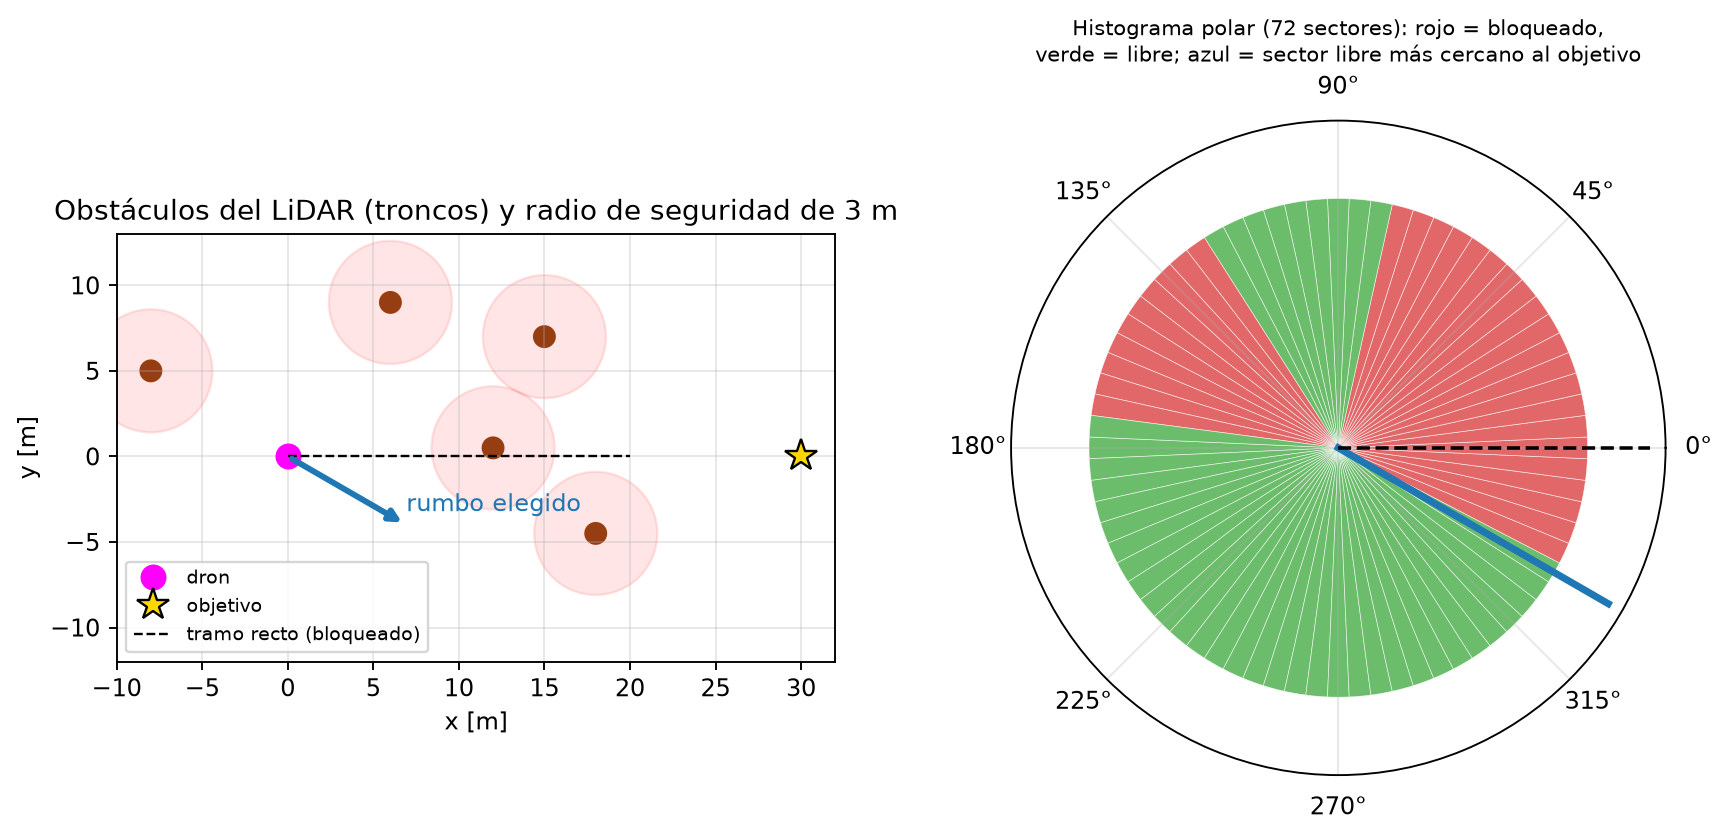
\includegraphics[width=\textwidth]{vfh.png}
\caption{Evasión con histograma polar.}
\end{figure}

Para las montañas no hace falta el LiDAR: el relieve se conoce (el DEM), así que el dron sube antes de
llegar a una ladera. El capítulo siguiente cuenta cómo se juntaron todas estas piezas.
